\documentclass[aspectratio=169]{beamer}

% ============================================================
% THEME AND PACKAGES
% ============================================================
\usetheme{metropolis}
\usepackage[utf8]{inputenc}
\usepackage[T1]{fontenc}
\usepackage[english]{babel}
\usepackage{graphicx}
\usepackage{booktabs}
\usepackage{xcolor}
\usepackage{tikz}
\usepackage{pgfplots}
\pgfplotsset{compat=1.18}
\usepackage[edges]{forest}
\usetikzlibrary{shapes,arrows,positioning,fit,backgrounds,calc,decorations.pathreplacing}
\usepackage{tcolorbox}
\tcbuselibrary{skins,breakable,listings}
\usepackage{setspace}
\usepackage{microtype}
\usepackage{listings}
\usepackage{hyperref}

% ============================================================
% COLOR SCHEME
% ============================================================
\definecolor{primarydark}{RGB}{15,23,42}
\definecolor{primaryblue}{RGB}{30,64,175}
\definecolor{accentcyan}{RGB}{6,182,212}
\definecolor{accentorange}{RGB}{251,146,60}
\definecolor{accentred}{RGB}{239,68,68}
\definecolor{accentgreen}{RGB}{34,197,94}
\definecolor{accentpurple}{RGB}{168,85,247}
\definecolor{lightgray}{RGB}{241,245,249}
\definecolor{textgray}{RGB}{71,85,105}
\definecolor{rustcolor}{RGB}{183,65,14}
\definecolor{pythoncolor}{RGB}{55,118,171}

\definecolor{chartcolor1}{RGB}{231,76,60}
\definecolor{chartcolor2}{RGB}{52,152,219}
\definecolor{chartcolor3}{RGB}{46,204,113}
\definecolor{chartcolor4}{RGB}{241,196,15}
\definecolor{chartcolor5}{RGB}{155,89,182}
\definecolor{chartcolor6}{RGB}{230,126,34}

% ============================================================
% BEAMER THEME CONFIGURATION
% ============================================================
\setbeamercolor{normal text}{fg=primarydark,bg=white}
\setbeamercolor{alerted text}{fg=accentred}
\setbeamercolor{example text}{fg=accentgreen}
\setbeamercolor{frametitle}{bg=primarydark,fg=white}
\setbeamercolor{title separator}{fg=accentcyan}
\setbeamercolor{progress bar}{fg=accentcyan,bg=primarydark!20}
\setbeamercolor{block title}{fg=white,bg=primaryblue}
\setbeamercolor{block body}{fg=primarydark,bg=lightgray}
\setbeamercolor{block title alerted}{fg=white,bg=accentred}
\setbeamercolor{block body alerted}{fg=primarydark,bg=accentred!8}
\setbeamercolor{block title example}{fg=white, bg=rustcolor}
\setbeamercolor{block body example}{bg=rustcolor!8}
\setbeamercolor{itemize item}{fg=primaryblue}
\setbeamercolor{enumerate item}{fg=primaryblue}

\metroset{
  titleformat=regular,
  sectionpage=progressbar,
  numbering=fraction,
  progressbar=frametitle,
  block=fill
}

% ============================================================
% LISTINGS CONFIGURATION
% ============================================================
\lstdefinestyle{ruststyle}{
  language=C,
  basicstyle=\ttfamily\scriptsize,
  keywordstyle=\color{primaryblue}\bfseries,
  stringstyle=\color{accentgreen!80!black},
  commentstyle=\color{textgray}\itshape,
  showstringspaces=false,
  breaklines=true,
  frame=none,
  backgroundcolor=\color{lightgray},
  morekeywords={fn,let,mut,pub,use,mod,struct,impl,const,match,Ok,Err,Some,None,Result,self,crate,if,else,loop,break,return,where,for,in,true,false,String,Vec,Path,PathBuf,u8,u16,u32,u64,bool},
  literate={->}{{$\rightarrow$}}1 {=>}{{$\Rightarrow$}}1,
}

\lstdefinestyle{pythonstyle}{
  language=Python,
  basicstyle=\ttfamily\scriptsize,
  keywordstyle=\color{pythoncolor}\bfseries,
  stringstyle=\color{accentgreen!80!black},
  commentstyle=\color{textgray}\itshape,
  showstringspaces=false,
  breaklines=true,
  frame=none,
  backgroundcolor=\color{lightgray},
}

% ============================================================
% CUSTOM BOXES
% ============================================================
\newtcolorbox{codebox}[1]{
  enhanced,
  colback=white,
  colframe=primaryblue,
  colbacktitle=primaryblue,
  coltitle=white,
  coltext=primarydark,
  title={\textbf{#1}},
  fonttitle=\sffamily\bfseries\small,
  fontupper=\sffamily\footnotesize,
  arc=3pt,
  boxrule=0pt,
  leftrule=3pt,
  toptitle=4pt,
  bottomtitle=4pt,
  left=8pt, right=8pt, top=4pt, bottom=6pt,
  before skip=6pt,
  after skip=6pt
}

\newtcolorbox{infobox}[1]{
  enhanced,
  colback=accentcyan!5,
  colframe=accentcyan,
  coltext=primarydark,
  title={\textbf{#1}},
  coltitle=white,
  colbacktitle=accentcyan,
  fonttitle=\sffamily\bfseries\small,
  fontupper=\sffamily\footnotesize,
  arc=3pt,
  boxrule=0pt,
  leftrule=3pt,
  toptitle=5pt,
  bottomtitle=5pt,
  left=8pt, right=8pt, top=4pt, bottom=6pt,
  before skip=6pt,
  after skip=6pt
}

\newtcolorbox{warnbox}[1]{
  enhanced,
  colback=accentorange!8,
  colframe=accentorange,
  coltext=primarydark,
  title={\textbf{#1}},
  coltitle=accentorange!80!black,
  colbacktitle=accentorange!25,
  fonttitle=\sffamily\bfseries\small,
  fontupper=\sffamily\footnotesize,
  arc=3pt,
  boxrule=0pt,
  leftrule=3pt,
  toptitle=5pt,
  bottomtitle=5pt,
  left=8pt, right=8pt, top=4pt, bottom=6pt,
  before skip=6pt,
  after skip=6pt
}

\newtcolorbox{dangerbox}[1]{
  enhanced,
  colback=accentred!5,
  colframe=accentred,
  coltext=primarydark,
  title={\textbf{#1}},
  coltitle=white,
  colbacktitle=accentred,
  fonttitle=\sffamily\bfseries\small,
  fontupper=\sffamily\footnotesize,
  arc=3pt,
  boxrule=0pt,
  leftrule=3pt,
  toptitle=5pt,
  bottomtitle=5pt,
  left=8pt, right=8pt, top=4pt, bottom=6pt,
  before skip=6pt,
  after skip=6pt
}

% ============================================================
% TYPOGRAPHY
% ============================================================
\setbeamerfont{title}{size=\LARGE,series=\bfseries}
\setbeamerfont{subtitle}{size=\normalsize}
\setbeamerfont{frametitle}{size=\large,series=\bfseries}
\setbeamerfont{block title}{size=\small,series=\bfseries}

\setlength{\leftmargini}{1em}
\setlength{\leftmarginii}{0.8em}

\newcommand{\code}[1]{\texttt{\textcolor{primaryblue}{#1}}}
\newcommand{\rustbadge}{\textcolor{rustcolor}{\textbf{Rust}}}
\newcommand{\pythonbadge}{\textcolor{pythoncolor}{\textbf{Python}}}

% ============================================================
% TITLE PAGE
% ============================================================
\title{Edu-Ransomware}
\subtitle{Architecture, Features, and Implementation Details}
\date{\today}
\institute{IT Security -- Educational Ransomware Simulation Project}

\begin{document}

% ============================================================
% TITLE SLIDE
% ============================================================
{
\setbeamertemplate{background}{
  \begin{tikzpicture}[overlay,remember picture]
    \shade[top color=primarydark,bottom color=primaryblue!50!primarydark]
      (current page.south west) rectangle (current page.north east);
    \draw[accentcyan,line width=2pt]
      ([yshift=-0.5cm]current page.center) ++(-5,0) -- ++(10,0);
  \end{tikzpicture}
}
\setbeamercolor{title}{fg=white}
\setbeamercolor{subtitle}{fg=accentcyan}
\setbeamercolor{institute}{fg=white!60}
\setbeamercolor{date}{fg=white!60}
\begin{frame}[plain]
  \vspace{2cm}
  \begin{center}
    {\usebeamerfont{title}\usebeamercolor[fg]{title}\inserttitle}\\[0.8em]
    {\usebeamerfont{subtitle}\usebeamercolor[fg]{subtitle}\insertsubtitle}\\[1.5em]
    {\footnotesize\usebeamercolor[fg]{institute}\insertinstitute}\\[0.3em]
    {\footnotesize\usebeamercolor[fg]{date}\insertdate}
  \end{center}
\end{frame}
}

% ============================================================
% DISCLAIMER
% ============================================================
\begin{frame}{Legal Disclaimer}
  \begin{dangerbox}{Important Notice}
    This software was developed \textbf{exclusively for educational purposes} and security research.

    \vspace{0.3em}
    \begin{itemize}
      \item Using this software on systems without explicit authorization is \textbf{illegal}.
      \item \textbf{NEVER} run this malware on production systems.
      \item Always use an isolated Virtual Machine (VM).
      \item The Pinggy tunnel links expire after 60 minutes as a safety mechanism.
    \end{itemize}
  \end{dangerbox}

  \vspace{0.5em}
  \begin{center}
    \textbf{Repository:} \url{https://github.com/TimBLukas/rust-mw}\\[0.3em]
    \textbf{License:} MIT (with Ethical Use Clause)
  \end{center}
\end{frame}

% ============================================================
% AGENDA
% ============================================================
\begin{frame}{Agenda}
  \tableofcontents
\end{frame}

% ============================================================
% SECTION 1: PROJECT OVERVIEW
% ============================================================
\section{Project Overview}

\begin{frame}[fragile]{What is Edu-Ransomware?}
  \begin{columns}[T]
    \begin{column}{0.55\textwidth}
      \textbf{A full-stack ransomware simulation} built for educational purposes to demonstrate how modern ransomware attacks work end-to-end.

      \vspace{0.5em}
      \textbf{Components:}
      \begin{enumerate}
        \item \rustbadge{} \textbf{Malware Agent} -- Executes on victim system
        \item \pythonbadge{} \textbf{C2 Server} -- Command and control
        \item \pythonbadge{} \textbf{Delivery Server} -- Drive-by-download
        \item \pythonbadge{} \textbf{PDF Phishing} -- Social engineering
      \end{enumerate}

      \vspace{0.5em}
      \textbf{Goal:} Investigate how complex it is for beginners to create functional ransomware with modern tools and AI assistance.
    \end{column}
    \begin{column}{0.42\textwidth}
      \centering
      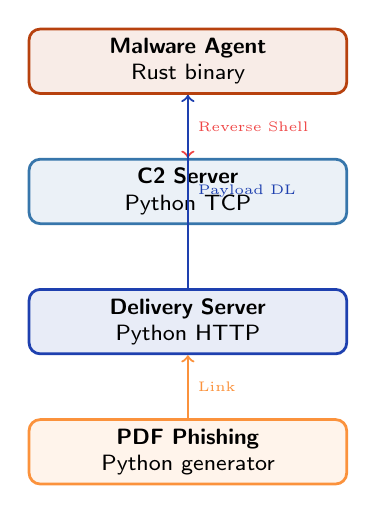
\begin{tikzpicture}[font=\sffamily\footnotesize, node distance=0.8cm]
        \node[rectangle, draw=rustcolor, fill=rustcolor!10, text width=3.8cm, align=center, rounded corners, line width=1pt] (agent) {\textbf{Malware Agent}\\Rust binary};
        \node[rectangle, draw=pythoncolor, fill=pythoncolor!10, text width=3.8cm, align=center, rounded corners, line width=1pt, below=of agent] (c2) {\textbf{C2 Server}\\Python TCP};
        \node[rectangle, draw=primaryblue, fill=primaryblue!10, text width=3.8cm, align=center, rounded corners, line width=1pt, below=of c2] (delivery) {\textbf{Delivery Server}\\Python HTTP};
        \node[rectangle, draw=accentorange, fill=accentorange!10, text width=3.8cm, align=center, rounded corners, line width=1pt, below=of delivery] (pdf) {\textbf{PDF Phishing}\\Python generator};

        \draw[->, thick, accentred] (agent) -- node[right, font=\tiny] {Reverse Shell} (c2);
        \draw[->, thick, primaryblue] (delivery) -- node[right, font=\tiny] {Payload DL} (agent);
        \draw[->, thick, accentorange] (pdf) -- node[right, font=\tiny] {Link} (delivery);
      \end{tikzpicture}
    \end{column}
  \end{columns}
\end{frame}

\begin{frame}{Technology Stack}
  \begin{columns}[T]
    \begin{column}{0.48\textwidth}
      \begin{exampleblock}{Malware Agent -- \rustbadge}
        \footnotesize
        \textbf{Why Rust?}
        \begin{itemize}
          \item Compiles to native static binary (no runtime needed)
          \item Cross-compilation: Windows, Linux, macOS from one codebase
          \item Memory safety without garbage collector
          \item Complex binaries are harder to reverse-engineer
          \item Growing trend in real-world malware (BlackCat/ALPHV)
        \end{itemize}

        \vspace{0.3em}
        \textbf{Key Crates:}
        \begin{itemize}
          \item \code{aes}, \code{ctr} -- AES-256-CTR encryption
          \item \code{walkdir} -- Recursive filesystem traversal
          \item \code{sysinfo} -- System information queries
          \item \code{wallpaper} -- Desktop wallpaper manipulation
          \item \code{base64} -- Data encoding for exfiltration
        \end{itemize}
      \end{exampleblock}
    \end{column}
    \begin{column}{0.48\textwidth}
      \begin{block}{C2 Server -- \pythonbadge}
        \footnotesize
        \begin{itemize}
          \item Multithreaded TCP socket server
          \item Interactive CLI for operator control
          \item Base64 stream decoding for exfiltration
          \item Session management for multiple victims
          \item ANSI-colored terminal output
        \end{itemize}
      \end{block}

      \vspace{0.3em}
      \begin{block}{Infrastructure}
        \footnotesize
        \begin{itemize}
          \item \textbf{Tunneling:} Pinggy.io TCP tunnels (NAT traversal)
          \item \textbf{Delivery:} Python HTTP server with OS detection
          \item \textbf{Build:} Cargo cross-compilation + shell scripts
          \item \textbf{Containerization:} Docker / Docker Compose
        \end{itemize}
      \end{block}
    \end{column}
  \end{columns}
\end{frame}

% ============================================================
% SECTION 2: SYSTEM ARCHITECTURE
% ============================================================
\section{System Architecture}

\begin{frame}[fragile]{High-Level Architecture}
  \centering
  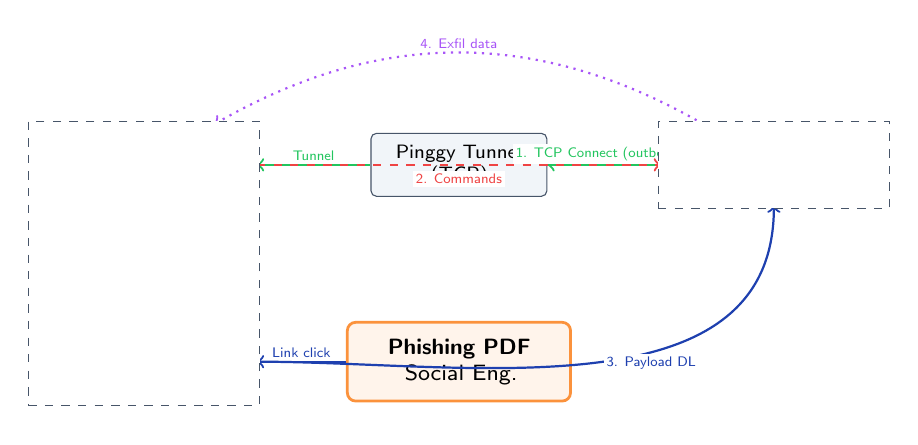
\begin{tikzpicture}[
    component/.style={rectangle, draw=#1, fill=#1!10, minimum width=2.8cm, minimum height=1cm, text width=2.6cm, align=center, font=\footnotesize\sffamily, rounded corners=3pt, line width=1pt},
    infra/.style={rectangle, draw=textgray, fill=lightgray, minimum width=2.2cm, minimum height=0.8cm, text width=2cm, align=center, font=\scriptsize\sffamily, rounded corners=2pt},
    arrow/.style={->, thick, #1},
    label/.style={font=\tiny\sffamily, fill=white, inner sep=1pt}
  ]
    % Attacker side
    \node[component=pythoncolor] (c2) at (0, 0) {\textbf{C2 Server}\\Python:4444};
    \node[component=primaryblue] (delivery) at (0, -2.5) {\textbf{Delivery Server}\\Python:3000};
    \node[infra] (tunnel) at (4, 0) {Pinggy Tunnel\\(TCP)};

    % Victim side
    \node[component=rustcolor] (agent) at (8, 0) {\textbf{Rust Agent}\\(Victim PC)};
    \node[component=accentorange] (pdf) at (4, -2.5) {\textbf{Phishing PDF}\\Social Eng.};

    % Connections
    \draw[arrow=accentgreen] (agent) -- node[label, above] {1. TCP Connect (outbound)} (tunnel);
    \draw[arrow=accentgreen] (tunnel) -- node[label, above] {Tunnel} (c2);
    \draw[arrow=accentred, dashed] (c2) -- node[label, below, yshift=-2pt] {2. Commands} (agent);

    \draw[arrow=primaryblue] (pdf) -- node[label, above] {Link click} (delivery);
    \draw[arrow=primaryblue] (delivery) to[out=0,in=-90] node[label, right, xshift=3pt] {3. Payload DL} (agent);

    % Data flow
    \draw[arrow=accentpurple, dotted, thick] (agent) to[out=150,in=30] node[label, above] {4. Exfil data} (c2);

    % Grouping
    \node[draw=textgray, dashed, fit=(c2)(delivery), inner sep=8pt, label={[font=\scriptsize\sffamily]above:Attacker Network}] {};
    \node[draw=textgray, dashed, fit=(agent), inner sep=12pt, label={[font=\scriptsize\sffamily]above:Victim Network}] {};
  \end{tikzpicture}
\end{frame}

\begin{frame}{Project Structure}
  \footnotesize
  \begin{columns}[T]
    \begin{column}{0.48\textwidth}
      \begin{forest}
        for tree={
          font=\ttfamily\scriptsize,
          grow'=0,
          child anchor=west,
          parent anchor=south,
          anchor=west,
          calign=first,
          edge path={
            \noexpand\path [draw, \forestoption{edge}]
            (!u.south west) +(7.5pt,0) |- node[fill,inner sep=1.25pt] {} (.child anchor)\forestoption{edge label};
          },
          before typesetting nodes={
            if n=1 {insert before={[,phantom]}} {}
          },
          fit=band,
          before computing xy={l=12pt},
        }
        [rust-mw/
          [malware\_agent/ \textcolor{rustcolor}{(Rust)}
            [src/
              [main.rs]
              [lib.rs]
              [config.rs]
              [crypto/ \textcolor{textgray}{(AES, Hybrid)}]
              [evasion/ \textcolor{textgray}{(HW, Behavior, Process)}]
              [network/ \textcolor{textgray}{(C2, DGA, Discovery, Exfil)}]
              [recon/ \textcolor{textgray}{(LDAP, SMB)}]
              [stealth/ \textcolor{textgray}{(Antiforensics, Mutex)}]
              [safety/ \textcolor{textgray}{(Killswitch, Geofencing)}]
              [persistence.rs]
              [extortion.rs]
            ]
          ]
        ]
      \end{forest}
    \end{column}
    \begin{column}{0.48\textwidth}
      \begin{forest}
        for tree={
          font=\ttfamily\scriptsize,
          grow'=0,
          child anchor=west,
          parent anchor=south,
          anchor=west,
          calign=first,
          edge path={
            \noexpand\path [draw, \forestoption{edge}]
            (!u.south west) +(7.5pt,0) |- node[fill,inner sep=1.25pt] {} (.child anchor)\forestoption{edge label};
          },
          before typesetting nodes={
            if n=1 {insert before={[,phantom]}} {}
          },
          fit=band,
          before computing xy={l=12pt},
        }
        [rust-mw/ (continued)
          [c2\_server/ \textcolor{pythoncolor}{(Python)}
            [server.py]
            [loot/]
          ]
          [delivery/ \textcolor{pythoncolor}{(Python)}
            [DbD-Site/
              [server.py]
              [public/ \textcolor{textgray}{(HTML templates)}]
              [files/ \textcolor{textgray}{(Payloads)}]
            ]
            [pdf\_phishing/]
          ]
          [scripts/]
          [Dockerfile]
          [docker-compose.yml]
        ]
      \end{forest}
    \end{column}
  \end{columns}
\end{frame}

\begin{frame}[fragile]{Modular Agent Architecture}
  \centering
  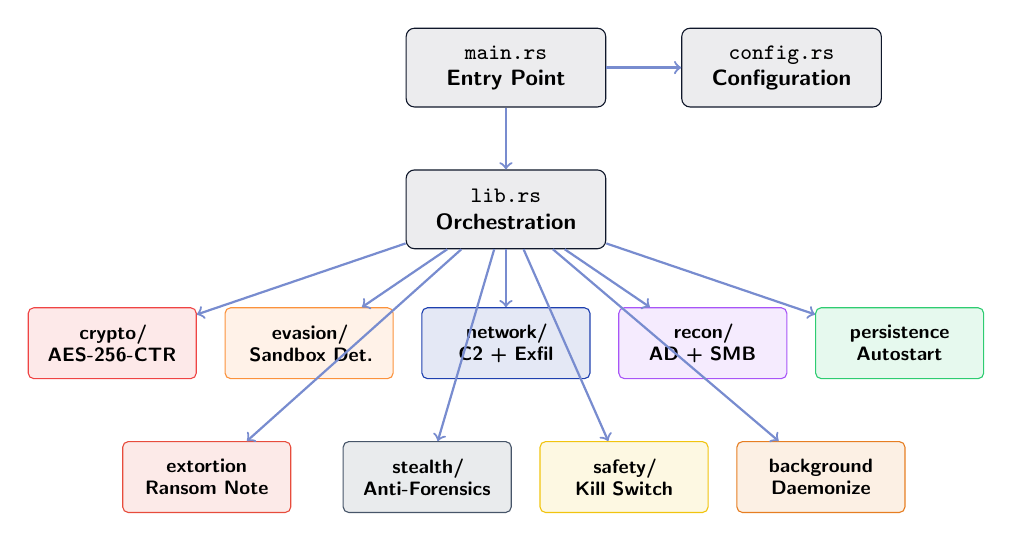
\begin{tikzpicture}[
    module/.style={rectangle, draw=#1, fill=#1!12, minimum width=2cm, minimum height=0.9cm, text width=1.9cm, align=center, font=\scriptsize\sffamily\bfseries, rounded corners=2pt},
    core/.style={rectangle, draw=primarydark, fill=primarydark!8, minimum width=2.5cm, minimum height=1cm, text width=2.3cm, align=center, font=\footnotesize\sffamily\bfseries, rounded corners=3pt},
    arrow/.style={->, thick, primaryblue!60}
  ]
    % Core
    \node[core] (main) at (0, 0) {\texttt{main.rs}\\Entry Point};
    \node[core] (lib) at (0, -1.8) {\texttt{lib.rs}\\Orchestration};
    \node[core] (config) at (3.5, 0) {\texttt{config.rs}\\Configuration};

    % Modules around
    \node[module=accentred] (crypto) at (-5, -3.5) {crypto/\\AES-256-CTR};
    \node[module=accentorange] (evasion) at (-2.5, -3.5) {evasion/\\Sandbox Det.};
    \node[module=primaryblue] (network) at (0, -3.5) {network/\\C2 + Exfil};
    \node[module=accentpurple] (recon) at (2.5, -3.5) {recon/\\AD + SMB};
    \node[module=chartcolor3] (persist) at (5, -3.5) {persistence\\Autostart};

    \node[module=chartcolor1] (extort) at (-3.8, -5.2) {extortion\\Ransom Note};
    \node[module=textgray] (stealth) at (-1, -5.2) {stealth/\\Anti-Forensics};
    \node[module=chartcolor4] (safety) at (1.5, -5.2) {safety/\\Kill Switch};
    \node[module=chartcolor6] (bg) at (4, -5.2) {background\\Daemonize};

    % Connections
    \draw[arrow] (main) -- (lib);
    \draw[arrow] (main) -- (config);
    \draw[arrow] (lib) -- (crypto);
    \draw[arrow] (lib) -- (evasion);
    \draw[arrow] (lib) -- (network);
    \draw[arrow] (lib) -- (recon);
    \draw[arrow] (lib) -- (persist);
    \draw[arrow] (lib) -- (extort);
    \draw[arrow] (lib) -- (stealth);
    \draw[arrow] (lib) -- (safety);
    \draw[arrow] (lib) -- (bg);
  \end{tikzpicture}
\end{frame}

% ============================================================
% SECTION 3: ATTACK KILL CHAIN
% ============================================================
\section{Attack Kill Chain}

\begin{frame}{Attack Flow -- Code Walkthrough}
  \textbf{Execution sequence of the Rust agent (\code{main.rs}):}

  \vspace{0.5em}
  \begin{enumerate}
    \item \textbf{Daemonize} (\code{background.rs})
    \begin{itemize}
      \item Linux: \code{fork()} to background; Windows: \code{windows\_subsystem} attribute
    \end{itemize}

    \item \textbf{Sandbox Detection} (\code{evasion/})
    \begin{itemize}
      \item \textbf{Pass:} Environment appears safe $\rightarrow$ continue
      \item \textbf{Fail:} Fake error message $\rightarrow$ \textbf{exit immediately}
    \end{itemize}

    \item \textbf{Establish Persistence} (\code{persistence.rs})
    \begin{itemize}
      \item Set up autostart to survive reboots
    \end{itemize}

    \item \textbf{C2 Loop} (\code{network/c2.rs})
    \begin{itemize}
      \item Connect to C2 server, await commands
    \end{itemize}

    \item \textbf{On Command: Encrypt} (\code{crypto/aes.rs})
    \begin{itemize}
      \item AES-256-CTR encryption of target directory
    \end{itemize}

    \item \textbf{On Command: Extort} (\code{extortion.rs})
    \begin{itemize}
      \item Deploy ransom note, change wallpaper
    \end{itemize}
  \end{enumerate}
\end{frame}

% ============================================================
% SECTION 4: DELIVERY MECHANISMS
% ============================================================
\section{Delivery Mechanisms}

\begin{frame}[fragile]{Drive-by Download}
  \begin{columns}[T]
    \begin{column}{0.55\textwidth}
      \textbf{Smart payload delivery based on OS detection:}

      \vspace{0.5em}
      The delivery server (\code{delivery/DbD-Site/server.py}) provides:
      \begin{itemize}
        \item Multiple phishing page templates:
        \begin{itemize}
          \item \code{/game} -- Fake gaming download
          \item \code{/security} -- Fake security alert
          \item \code{/prize} -- Fake prize notification
        \end{itemize}
        \item \code{/get\_document} -- Smart download endpoint
        \item \textbf{User-Agent detection:} Identifies Windows, Linux, or macOS
        \item Delivers OS-specific payload automatically
      \end{itemize}

      \vspace{0.3em}
      \begin{infobox}{Build Pipeline}
        \code{build\_payloads.sh} cross-compiles the Rust agent for all platforms and copies binaries to \code{delivery/DbD-Site/files/}.
      \end{infobox}
    \end{column}
    \begin{column}{0.42\textwidth}
      \centering
      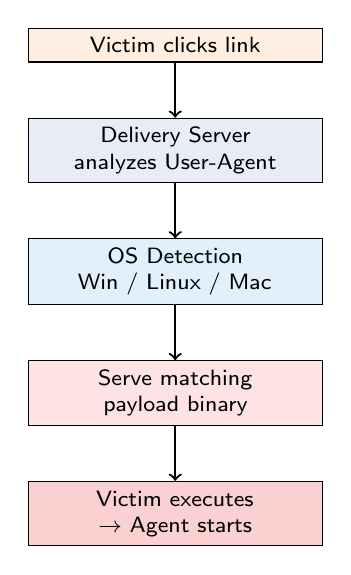
\begin{tikzpicture}[font=\sffamily\footnotesize, node distance=0.7cm]
        \node[rectangle, draw, fill=accentorange!15, text width=3.5cm, align=center] (victim) {Victim clicks link};
        \node[rectangle, draw, fill=primaryblue!10, text width=3.5cm, align=center, below=of victim] (server) {Delivery Server\\analyzes User-Agent};
        \node[rectangle, draw, fill=chartcolor2!15, text width=3.5cm, align=center, below=of server] (detect) {OS Detection\\Win / Linux / Mac};
        \node[rectangle, draw, fill=accentred!15, text width=3.5cm, align=center, below=of detect] (payload) {Serve matching\\payload binary};
        \node[rectangle, draw, fill=accentred!25, text width=3.5cm, align=center, below=of payload] (exec) {Victim executes\\$\rightarrow$ Agent starts};

        \draw[->, thick] (victim) -- (server);
        \draw[->, thick] (server) -- (detect);
        \draw[->, thick] (detect) -- (payload);
        \draw[->, thick] (payload) -- (exec);
      \end{tikzpicture}
    \end{column}
  \end{columns}
\end{frame}

\begin{frame}[fragile]{PDF Phishing}
  \begin{columns}[T]
    \begin{column}{0.55\textwidth}
      \textbf{Social engineering via crafted PDF:}

      \vspace{0.5em}
      \begin{itemize}
        \item Generated by \code{delivery/pdf\_phishing/generate\_phishing\_pdf.py}
        \item Contains a \textbf{blurred invoice image} as bait
        \item Button labeled ``Decrypt Content'' (social engineering)
        \item Clicking the button opens the delivery server URL
        \item Delivery server then serves the OS-specific malware
      \end{itemize}

      \vspace{0.5em}
      \textbf{Attack scenario:}
      \begin{enumerate}
        \item Employee receives email with \code{Invoice\_Dec.pdf}
        \item Opens PDF, sees blurred invoice
        \item Clicks ``Decrypt Content'' button
        \item Browser opens $\rightarrow$ Delivery server detects OS
        \item Malware binary downloads and executes
      \end{enumerate}
    \end{column}
    \begin{column}{0.42\textwidth}
      \centering
      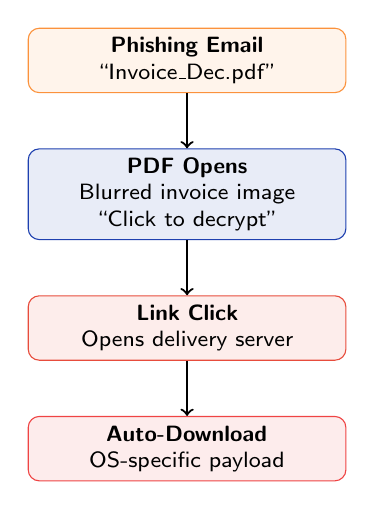
\begin{tikzpicture}[font=\sffamily\footnotesize, node distance=0.7cm]
        \node[rectangle, draw=accentorange, fill=accentorange!10, text width=3.8cm, align=center, rounded corners] (email) {\textbf{Phishing Email}\\``Invoice\_Dec.pdf''};
        \node[rectangle, draw=primaryblue, fill=primaryblue!10, text width=3.8cm, align=center, rounded corners, below=of email] (pdf) {\textbf{PDF Opens}\\Blurred invoice image\\``Click to decrypt''};
        \node[rectangle, draw=chartcolor1, fill=chartcolor1!10, text width=3.8cm, align=center, rounded corners, below=of pdf] (link) {\textbf{Link Click}\\Opens delivery server};
        \node[rectangle, draw=accentred, fill=accentred!10, text width=3.8cm, align=center, rounded corners, below=of link] (dl) {\textbf{Auto-Download}\\OS-specific payload};

        \draw[->, thick] (email) -- (pdf);
        \draw[->, thick] (pdf) -- (link);
        \draw[->, thick] (link) -- (dl);
      \end{tikzpicture}
    \end{column}
  \end{columns}
\end{frame}

% ============================================================
% SECTION 5: EVASION MODULE
% ============================================================
\section{Evasion Module}

\begin{frame}{Multi-Layer Sandbox Detection}
  \textbf{Module: \code{evasion/} -- Checks run sequentially (fast checks first):}

  \vspace{0.5em}
  \begin{columns}[T]
    \begin{column}{0.32\textwidth}
      \begin{block}{1. Hardware Checks \\ \footnotesize\code{hardware.rs}}
        \footnotesize
        \begin{itemize}
          \item RAM $<$ 3 GB? $\rightarrow$ VM/Sandbox
          \item CPU cores $<$ 3? $\rightarrow$ VM
          \item Disk space $<$ 60 GB? $\rightarrow$ VM
        \end{itemize}
        \vspace{0.3em}
        \textit{Uses \code{sysinfo} crate for cross-platform system queries.}
      \end{block}
    \end{column}
    \begin{column}{0.32\textwidth}
      \begin{block}{2. Process Scan \\ \footnotesize\code{process.rs}}
        \footnotesize
        Checks for analysis tools:
        \begin{itemize}
          \item Wireshark
          \item Process Monitor
          \item x64dbg / OllyDbg
          \item Fiddler
          \item IDA Pro
        \end{itemize}
        \textit{If found: immediate exit.}
      \end{block}
    \end{column}
    \begin{column}{0.32\textwidth}
      \begin{block}{3. Behavior Check \\ \footnotesize\code{behavior.rs}}
        \footnotesize
        \begin{itemize}
          \item Record mouse position
          \item Sleep for 5 seconds
          \item Record mouse position again
          \item If no movement: \alert{sandbox!}
          \item Also detects sleep acceleration
        \end{itemize}
        \textit{Run last (slowest check).}
      \end{block}
    \end{column}
  \end{columns}

  \vspace{0.5em}
  \begin{warnbox}{On Detection}
    If any check fails, the agent prints a fake error: \code{"Error: Runtime failed to initialize required components (0xC0000005)."} and exits with code 1.
  \end{warnbox}
\end{frame}

% ============================================================
% SECTION 6: NETWORK COMMUNICATION
% ============================================================
\section{Network Communication}

\begin{frame}[fragile]{Reverse Shell Architecture}
  \begin{columns}[T]
    \begin{column}{0.45\textwidth}
      \textbf{Why reverse shell?}
      \begin{itemize}
        \item Victim connects \textbf{outward} to attacker
        \item Bypasses firewall rules (outbound traffic typically allowed)
        \item NAT traversal via Pinggy.io TCP tunnel
      \end{itemize}

      \vspace{0.5em}
      \textbf{Connection Flow:}
      \begin{enumerate}
        \item Agent reads C2 address from \code{config.rs}
        \item Connects via \code{TcpStream::connect()}
        \item Enters command loop: receive $\rightarrow$ execute $\rightarrow$ respond
        \item Retry logic: 5 attempts with 5s delay
        \item On exhaustion: silent exit
      \end{enumerate}

      \vspace{0.3em}
      \begin{infobox}{Safety Mechanism}
        Pinggy tunnel links expire after 60 minutes, rendering the malware inoperable.
      \end{infobox}
    \end{column}
    \begin{column}{0.52\textwidth}
      \centering
      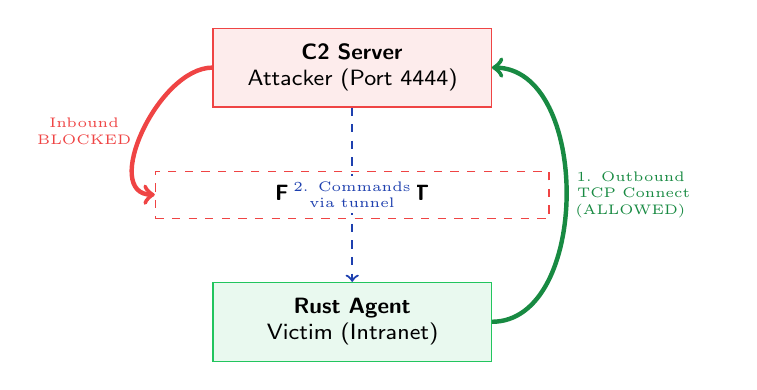
\begin{tikzpicture}[font=\sffamily\footnotesize, node distance=1.2cm]
        \node[rectangle, draw=accentred, fill=accentred!10, minimum width=3.5cm, minimum height=1cm, text width=3.3cm, align=center] (c2) {\textbf{C2 Server}\\Attacker (Port 4444)};

        \node[rectangle, draw=accentred, dashed, fill=white, minimum width=5cm, minimum height=0.6cm, below=0.8cm of c2] (fw) {\textbf{Firewall / NAT}};

        \node[rectangle, draw=accentgreen, fill=accentgreen!10, minimum width=3.5cm, minimum height=1cm, text width=3.3cm, align=center, below=0.8cm of fw] (agent) {\textbf{Rust Agent}\\Victim (Intranet)};

        % Outbound (allowed)
        \draw[->, ultra thick, accentgreen!70!black] (agent.east) to[out=0,in=0] node[right, font=\tiny, text width=1.8cm, align=left]{1. Outbound\\TCP Connect\\(ALLOWED)} (c2.east);

        % Inbound (blocked)
        \draw[->, ultra thick, accentred] (c2.west) to[out=180,in=180] node[left, font=\tiny, text width=1.2cm, align=center]{Inbound\\BLOCKED} (fw.west);

        % Response through tunnel
        \draw[->, thick, primaryblue, dashed] (c2) -- node[fill=white, font=\tiny, inner sep=2pt, text width=1.5cm, align=center]{2. Commands\\via tunnel} (agent);
      \end{tikzpicture}
    \end{column}
  \end{columns}
\end{frame}

\begin{frame}{C2 Command Set}
  \textbf{Commands processed by \code{network/c2.rs} $\rightarrow$ \code{process\_command\_logic()}:}

  \vspace{0.5em}
  \footnotesize
  \begin{tabular}{lll}
    \toprule
    \textbf{Command} & \textbf{Description} & \textbf{Module} \\
    \midrule
    \code{shell <cmd>} & Execute OS command on victim & \code{c2.rs} \\
    \code{encrypt [path]} & Encrypt target directory (AES-256-CTR) & \code{crypto/aes.rs} \\
    \code{decrypt [path]} & Decrypt \code{.locked} files using \code{rescue.key} & \code{crypto/aes.rs} \\
    \code{exfil <file>} & Exfiltrate single file (Base64-encoded) & \code{c2.rs} \\
    \code{auto-exfil} & Auto-exfiltrate high-value files (background) & \code{exfiltration.rs} \\
    \code{exfil-screenshot} & Capture and exfiltrate screenshot & \code{exfiltration.rs} \\
    \code{recon} & AD/LDAP + SMB network reconnaissance & \code{recon/} \\
    \code{kill} & Self-destruct: delete traces + exit & \code{stealth/} \\
    \bottomrule
  \end{tabular}

  \vspace{0.5em}
  \begin{columns}[T]
    \begin{column}{0.48\textwidth}
      \begin{infobox}{Fallback Behavior}
        Any unrecognized command is passed to the OS shell (\code{sh -c} on Linux, \code{cmd /C} on Windows) and output is returned to C2.
      \end{infobox}
    \end{column}
    \begin{column}{0.48\textwidth}
      \begin{codebox}{C2 Server CLI}
        \code{sessions} -- List connected victims\\
        \code{interact <id>} -- Interactive shell\\
        \code{broadcast <cmd>} -- Send to all victims
      \end{codebox}
    \end{column}
  \end{columns}
\end{frame}

% ============================================================
% SECTION 7: ENCRYPTION ENGINE
% ============================================================
\section{Encryption Engine}

\begin{frame}[fragile]{AES-256-CTR Atomic Encryption}
  \begin{columns}[T]
    \begin{column}{0.52\textwidth}
      \textbf{Module: \code{crypto/aes.rs}}

      \vspace{0.5em}
      \textbf{Algorithm:} AES-256 in CTR (Counter) mode
      \begin{itemize}
        \item Stream cipher -- processes data in chunks (4 KB)
        \item Symmetric key: 32 bytes (256 bits), randomly generated
        \item IV: 16 bytes (currently static for simplicity)
        \item Key saved to \code{rescue.key} in target directory
      \end{itemize}

      \vspace{0.5em}
      \textbf{Atomic file operation:}
      \begin{enumerate}
        \item Open original file for reading
        \item Create temp file (\code{.enc\_temp})
        \item Stream-encrypt chunks into temp file
        \item \textbf{Atomic rename:} temp $\rightarrow$ \code{.locked}
        \item Delete original file
      \end{enumerate}

      \vspace{0.3em}
      \begin{infobox}{Why Atomic?}
        If the process crashes mid-encryption, either the original or the encrypted file exists -- never a corrupted state.
      \end{infobox}
    \end{column}
    \begin{column}{0.45\textwidth}
      \centering
      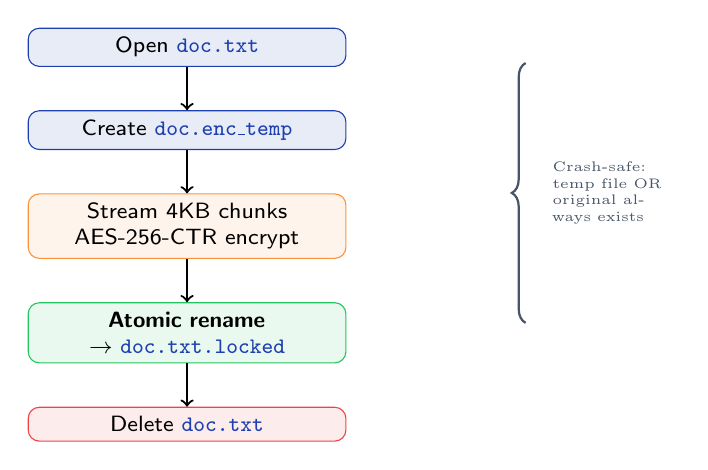
\begin{tikzpicture}[font=\sffamily\footnotesize, node distance=0.55cm]
        \node[rectangle, draw=primaryblue, fill=primaryblue!10, text width=3.8cm, align=center, rounded corners] (open) {Open \code{doc.txt}};
        \node[rectangle, draw=primaryblue, fill=primaryblue!10, text width=3.8cm, align=center, rounded corners, below=of open] (temp) {Create \code{doc.enc\_temp}};
        \node[rectangle, draw=accentorange, fill=accentorange!10, text width=3.8cm, align=center, rounded corners, below=of temp] (stream) {Stream 4KB chunks\\AES-256-CTR encrypt};
        \node[rectangle, draw=accentgreen, fill=accentgreen!10, text width=3.8cm, align=center, rounded corners, below=of stream] (rename) {\textbf{Atomic rename}\\$\rightarrow$ \code{doc.txt.locked}};
        \node[rectangle, draw=accentred, fill=accentred!10, text width=3.8cm, align=center, rounded corners, below=of rename] (delete) {Delete \code{doc.txt}};

        \draw[->, thick] (open) -- (temp);
        \draw[->, thick] (temp) -- (stream);
        \draw[->, thick] (stream) -- (rename);
        \draw[->, thick] (rename) -- (delete);

        % Annotation
        \draw[decorate, decoration={brace, amplitude=5pt, mirror}, thick, textgray] (4.3, -0.2) -- (4.3, -3.5) node[midway, right=6pt, font=\tiny, text width=1.5cm, align=left] {Crash-safe: temp file OR original always exists};
      \end{tikzpicture}
    \end{column}
  \end{columns}
\end{frame}

\begin{frame}{Encryption Orchestration}
  \textbf{Module: \code{lib.rs} $\rightarrow$ \code{run\_malware\_logic()}}

  \vspace{0.5em}
  \begin{columns}[T]
    \begin{column}{0.55\textwidth}
      \textbf{Full encryption workflow:}
      \begin{enumerate}
        \item Validate target directory exists
        \item Create and show ransom note (\code{README\_DECRYPT.html})
        \item Generate random AES-256 key
        \item Save key to \code{rescue.key}
        \item Walk filesystem recursively (\code{walkdir})
        \item For each file:
        \begin{itemize}
          \item Skip: \code{rescue.key}, \code{README\_DECRYPT.html}, \code{.locked}, \code{.enc\_temp}
          \item Encrypt with \code{encrypt\_file\_atomic()}
        \end{itemize}
        \item Change desktop wallpaper to ransom image
        \item Open ransom note in default browser
      \end{enumerate}
    \end{column}
    \begin{column}{0.42\textwidth}
      \textbf{Decryption (\code{run\_decryption\_logic}):}
      \begin{enumerate}
        \item Read \code{rescue.key} from target dir
        \item Validate key length (32 bytes)
        \item Walk filesystem for \code{.locked} files
        \item Decrypt each with same AES-CTR key
        \item Restore original filename
        \item Delete \code{.locked} file
      \end{enumerate}

      \vspace{0.5em}
      \begin{warnbox}{Symmetric Key on Disk}
        In this educational version, the key remains on disk (\code{rescue.key}). Real ransomware uses hybrid encryption (RSA wrapping) to prevent local recovery.
      \end{warnbox}
    \end{column}
  \end{columns}
\end{frame}

% ============================================================
% SECTION 8: PERSISTENCE MECHANISMS
% ============================================================
\section{Persistence Mechanisms}

\begin{frame}{Cross-Platform Persistence}
  \textbf{Module: \code{persistence.rs} -- Survives system reboots on all platforms:}

  \vspace{0.5em}
  \begin{columns}[T]
    \begin{column}{0.32\textwidth}
      \begin{block}{Linux (Dual Method)}
        \footnotesize
        \textbf{Method A: Systemd User Service}
        \begin{itemize}
          \item Creates \code{.service} file in \code{\textasciitilde/.config/systemd/user/}
          \item Type: \code{forking}
          \item Enabled via \code{systemctl --user}
          \item No root required
        \end{itemize}

        \vspace{0.3em}
        \textbf{Method B: Cron Job}
        \begin{itemize}
          \item Adds \code{@reboot} entry
          \item Reads existing crontab first
          \item Checks for duplicates
          \item Writes via \code{crontab -}
        \end{itemize}

        \textit{Both methods tried for redundancy.}
      \end{block}
    \end{column}
    \begin{column}{0.32\textwidth}
      \begin{block}{Windows (Dual Method)}
        \footnotesize
        \textbf{Method A: Scheduled Task}
        \begin{itemize}
          \item Uses \code{schtasks.exe}
          \item Trigger: \code{onlogon}
          \item Name: \code{WindowsUpdateHelper}
          \item Requests highest privileges
          \item \code{CREATE\_NO\_WINDOW} flag
        \end{itemize}

        \vspace{0.3em}
        \textbf{Method B: Registry Run Key}
        \begin{itemize}
          \item \code{HKCU\textbackslash...\textbackslash Run}
          \item Value: \code{SystemUpdater}
          \item Checked for existing entry
          \item Fallback if tasks fail
        \end{itemize}
      \end{block}
    \end{column}
    \begin{column}{0.32\textwidth}
      \begin{block}{macOS}
        \footnotesize
        \textbf{LaunchAgent}
        \begin{itemize}
          \item Creates \code{.plist} in \code{\textasciitilde/Library/LaunchAgents/}
          \item Label: \code{com.service.updater}
          \item \code{RunAtLoad: true}
          \item No root needed
        \end{itemize}
      \end{block}

      \vspace{0.3em}
      \begin{infobox}{Design Pattern}
        Uses \code{cfg!} compile-time conditionals to select OS-specific code. Each platform has an internal dispatch function and dedicated tests.
      \end{infobox}
    \end{column}
  \end{columns}
\end{frame}

% ============================================================
% SECTION 9: DATA EXFILTRATION
% ============================================================
\section{Data Exfiltration}

\begin{frame}{Exfiltration Capabilities}
  \textbf{Module: \code{network/exfiltration.rs} -- Double extortion support:}

  \vspace{0.5em}
  \begin{columns}[T]
    \begin{column}{0.48\textwidth}
      \begin{block}{Manual Exfiltration}
        \footnotesize
        \begin{itemize}
          \item C2 command: \code{exfil <filepath>}
          \item File read $\rightarrow$ Base64 encode $\rightarrow$ send
          \item Format: \code{EXFIL\_DATA:<filename>:<base64>}
          \item Server decodes and saves to \code{loot/} directory
        \end{itemize}
      \end{block}

      \vspace{0.3em}
      \begin{block}{Automated High-Value Exfiltration}
        \footnotesize
        Command: \code{auto-exfil}
        \begin{itemize}
          \item Runs in background thread (non-blocking)
          \item Searches for high-value files by keyword:
          \item \code{password}, \code{secret}, \code{iban}, \code{credit}
          \item File extensions: \code{.kdbx}, \code{.pem}, \code{.key}
          \item Opens separate TCP connection for transfer
        \end{itemize}
      \end{block}
    \end{column}
    \begin{column}{0.48\textwidth}
      \begin{block}{Screenshot Capture}
        \footnotesize
        Command: \code{exfil-screenshot}
        \begin{itemize}
          \item Captures screen using \code{screenshots} crate
          \item Encodes as PNG $\rightarrow$ Base64
          \item Sent via dedicated TCP connection
          \item Saved as image file in \code{loot/}
        \end{itemize}
      \end{block}

      \vspace{0.3em}
      \begin{infobox}{Server-Side Handling}
        The C2 server (\code{server.py}) uses a 1 MB receive buffer and accumulates chunks until transfer completes. Handles \code{EXFIL\_DATA} prefix parsing, Base64 decoding, and file saving automatically.
      \end{infobox}
    \end{column}
  \end{columns}
\end{frame}

% ============================================================
% SECTION 10: EXTORTION FEATURES
% ============================================================
\section{Extortion Features}

\begin{frame}{Visual Impact -- Ransom Note and Wallpaper}
  \textbf{Module: \code{extortion.rs} -- Maximum psychological pressure:}

  \vspace{0.5em}
  \begin{columns}[T]
    \begin{column}{0.48\textwidth}
      \begin{block}{Ransom Note (HTML)}
        \footnotesize
        \begin{itemize}
          \item File: \code{README\_DECRYPT.html}
          \item Full HTML/CSS with dark theme
          \item Red/black color scheme for urgency
          \item ``YOUR FILES ARE ENCRYPTED'' heading
          \item Instructions to contact C2 operator
          \item ``Decrypt Files Now'' button (opens alert)
          \item Auto-opened in default browser:
          \begin{itemize}
            \item Linux: \code{xdg-open}
            \item Windows: \code{cmd /C start}
            \item macOS: \code{open}
          \end{itemize}
        \end{itemize}
      \end{block}
    \end{column}
    \begin{column}{0.48\textwidth}
      \begin{block}{Desktop Wallpaper Change}
        \footnotesize
        \begin{itemize}
          \item Embedded image: \code{ransom\_wallpaper.jpg}
          \item Included at compile time via \code{include\_bytes!}
          \item Extracted to filesystem at runtime
          \item Set using \code{wallpaper} crate (cross-platform)
          \item Requires absolute path (\code{fs::canonicalize})
          \item Mode: Crop (fills entire screen)
        \end{itemize}
      \end{block}

      \vspace{0.3em}
      \begin{warnbox}{Psychological Effect}
        The combination of encrypted files, browser popup, and changed wallpaper creates immediate panic -- exactly what real ransomware aims to achieve to pressure victims into paying.
      \end{warnbox}
    \end{column}
  \end{columns}
\end{frame}

% ============================================================
% SECTION 11: RECONNAISSANCE
% ============================================================
\section{Network Reconnaissance}

\begin{frame}{Active Directory and SMB Reconnaissance}
  \textbf{Module: \code{recon/} -- Enterprise environment enumeration:}

  \vspace{0.5em}
  \begin{columns}[T]
    \begin{column}{0.48\textwidth}
      \begin{block}{LDAP Enumeration (\code{ldap.rs})}
        \footnotesize
        \begin{itemize}
          \item Auto-detects Domain Controller:
          \begin{itemize}
            \item Windows: \code{LOGONSERVER} env var
            \item Linux: \code{krb5.conf} / DNS SRV records
          \end{itemize}
          \item Enumerates without admin rights:
          \begin{itemize}
            \item Domain Admins group members
            \item Backup Operators
            \item All computer objects (FQDN)
            \item Domain Controller identification
          \end{itemize}
          \item Uses \code{ldap3} Rust crate
        \end{itemize}
      \end{block}
    \end{column}
    \begin{column}{0.48\textwidth}
      \begin{block}{SMB Share Enumeration (\code{smb.rs})}
        \footnotesize
        \begin{itemize}
          \item Cross-platform:
          \begin{itemize}
            \item Windows: \code{net view}
            \item Linux: \code{smbclient}
          \end{itemize}
          \item Port 445 connectivity check
          \item Read/write access testing
          \item Filters for encryption targets (writable disk shares)
          \item Subnet scanning for SMB hosts (\code{/24})
        \end{itemize}
      \end{block}

      \vspace{0.3em}
      \begin{block}{High-Value Target ID (\code{mod.rs})}
        \footnotesize
        Auto-detects critical systems by hostname patterns:\\
        DC, BACKUP, SQL, FILE, EXCHANGE, NAS, VEEAM, ADMIN
      \end{block}
    \end{column}
  \end{columns}

  \vspace{0.3em}
  \footnotesize
  \textbf{MITRE ATT\&CK:} T1069.002 (Domain Groups), T1087.002 (Domain Account), T1018 (Remote System Discovery), T1135 (Network Share Discovery)
\end{frame}

% ============================================================
% SECTION 12: SAFETY AND STEALTH
% ============================================================
\section{Safety and Stealth Features}

\begin{frame}{Safety Mechanisms}
  \textbf{Built-in safeguards to prevent accidental harm:}

  \vspace{0.5em}
  \begin{columns}[T]
    \begin{column}{0.48\textwidth}
      \begin{block}{Kill Switch (\code{safety/killswitch.rs})}
        \footnotesize
        \begin{itemize}
          \item HTTP check to remote URL before execution
          \item Response ``STOP'' $\rightarrow$ agent exits and self-deletes
          \item Response ``RUN'' or 404 $\rightarrow$ continue
          \item Configurable via \code{config.rs}
          \item Allows remote emergency shutdown
        \end{itemize}
      \end{block}

      \vspace{0.3em}
      \begin{block}{Geo-Fencing (\code{safety/geofencing.rs})}
        \footnotesize
        \begin{itemize}
          \item Checks local IP address
          \item Only allows private networks: \code{192.168.x.x}, \code{10.x.x.x}
          \item Prevents accidental execution on public networks
          \item Protects against ``zoo virus'' escaping the lab
        \end{itemize}
      \end{block}
    \end{column}
    \begin{column}{0.48\textwidth}
      \begin{block}{Singleton / Mutex (\code{stealth/mutex.rs})}
        \footnotesize
        \begin{itemize}
          \item Named lock prevents multiple instances
          \item Uses \code{named\_lock} crate
          \item If lock already held $\rightarrow$ exit silently
          \item Prevents double-encryption scenarios
        \end{itemize}
      \end{block}

      \vspace{0.3em}
      \begin{block}{Anti-Forensics (\code{stealth/antiforensics.rs})}
        \footnotesize
        \begin{itemize}
          \item \code{kill} command triggers full cleanup:
          \begin{itemize}
            \item Delete the executable itself
            \item Remove persistence entries
            \item Wipe shell history
            \item Symlink \code{.bash\_history} to \code{/dev/null}
          \end{itemize}
          \item Agent exits 500ms after cleanup
        \end{itemize}
      \end{block}
    \end{column}
  \end{columns}
\end{frame}

\begin{frame}[fragile]{Configuration System}
  \textbf{Module: \code{config.rs} -- Centralized compile-time configuration:}

  \vspace{0.5em}
  \begin{columns}[T]
    \begin{column}{0.55\textwidth}
      \begin{codebox}{Config Structure}
        \begin{lstlisting}[style=ruststyle]
pub struct Config {
    pub ip_adress: &'static str,
    pub port: u16,
    pub enable_evasion: bool,
    pub enable_killswitch: bool,
    pub safe_mode: bool,
}

impl Config {
    pub const fn default() -> Self {
        Config {
            ip_adress: CONFIG_IP_ADDR,
            port: CONFIG_PORT,
            enable_evasion: false,
            enable_killswitch: true,
            safe_mode: false,
        }
    }
}
        \end{lstlisting}
      \end{codebox}
    \end{column}
    \begin{column}{0.42\textwidth}
      \textbf{Configuration Fields:}

      \vspace{0.5em}
      \footnotesize
      \begin{tabular}{ll}
        \toprule
        \textbf{Field} & \textbf{Purpose} \\
        \midrule
        \code{ip\_adress} & C2 server hostname \\
        \code{port} & C2 server port \\
        \code{enable\_evasion} & Toggle sandbox checks \\
        \code{enable\_killswitch} & Toggle kill switch \\
        \code{safe\_mode} & Educational watermark \\
        \bottomrule
      \end{tabular}

      \vspace{0.5em}
      \begin{infobox}{Compile-Time Config}
        Uses \code{const fn} so the configuration is embedded at compile time. The Pinggy tunnel address must be updated before each build.
      \end{infobox}
    \end{column}
  \end{columns}
\end{frame}

% ============================================================
% SECTION 13: BACKGROUND AND STEALTH EXECUTION
% ============================================================
\section{Stealth Execution}

\begin{frame}{Background Execution and Window Hiding}
  \textbf{Module: \code{background.rs} -- Making the agent invisible:}

  \vspace{0.5em}
  \begin{columns}[T]
    \begin{column}{0.48\textwidth}
      \begin{block}{Linux: Process Daemonization}
        \footnotesize
        \begin{itemize}
          \item Uses \code{fork()} system call
          \item Parent process exits immediately
          \item Child continues in background
          \item Detached from terminal session
          \item No visible window or process name clue
          \item Standard daemon pattern
        \end{itemize}
      \end{block}
    \end{column}
    \begin{column}{0.48\textwidth}
      \begin{block}{Windows: Subsystem Trick}
        \footnotesize
        \begin{itemize}
          \item Compile-time attribute:\\
            \code{\#![windows\_subsystem = "windows"]}
          \item Tells Windows: ``this is a GUI app''
          \item No console window is created
          \item Process runs silently in background
          \item Invisible in taskbar
          \item Only visible in Task Manager
        \end{itemize}
      \end{block}
    \end{column}
  \end{columns}

  \vspace{0.5em}
  \begin{infobox}{Debug vs Release}
    The \code{windows\_subsystem} attribute is only active in release builds (\code{cfg(not(debug\_assertions))}). During development, a console window appears for debugging output.
  \end{infobox}
\end{frame}

% ============================================================
% SECTION 14: TESTING
% ============================================================
\section{Testing Strategy}

\begin{frame}{Comprehensive Test Suite}
  \textbf{Every module includes unit tests (\code{\#[cfg(test)]} blocks):}

  \vspace{0.5em}
  \begin{columns}[T]
    \begin{column}{0.48\textwidth}
      \begin{block}{Crypto Tests}
        \footnotesize
        \begin{itemize}
          \item Key generation (32-byte length, file persistence)
          \item Full encrypt/decrypt cycle (data integrity)
          \item Non-locked files are ignored during decryption
          \item Temp directory isolation for each test
        \end{itemize}
      \end{block}

      \vspace{0.3em}
      \begin{block}{Network Tests}
        \footnotesize
        \begin{itemize}
          \item Shell command execution (echo, error handling)
          \item Command parsing: encrypt, decrypt, exfil
          \item Custom path handling with trim
          \item Fallback to shell for unknown commands
          \item Auto-exfil and recon command recognition
        \end{itemize}
      \end{block}
    \end{column}
    \begin{column}{0.48\textwidth}
      \begin{block}{Extortion Tests}
        \footnotesize
        \begin{itemize}
          \item HTML content integrity checks
          \item File creation and path validation
          \item Content match: written vs.\ expected
          \item Permission error handling (invalid paths)
          \item Wallpaper function with missing files
        \end{itemize}
      \end{block}

      \vspace{0.3em}
      \begin{block}{Persistence Tests}
        \footnotesize
        \begin{itemize}
          \item Service file content generation
          \item Systemd file creation in temp dirs
          \item Cron entry string formatting
          \item macOS plist content validation
          \item Windows setup panic-free execution
          \item OS-specific conditional compilation (\code{\#[cfg]})
        \end{itemize}
      \end{block}
    \end{column}
  \end{columns}
\end{frame}

% ============================================================
% SECTION 15: MITRE ATT&CK MAPPING
% ============================================================
\section{MITRE ATT\&CK Mapping}

\begin{frame}{Tactics and Techniques Coverage}
  \footnotesize
  \begin{tabular}{llll}
    \toprule
    \textbf{Tactic} & \textbf{Technique} & \textbf{ID} & \textbf{Module} \\
    \midrule
    Initial Access & Drive-by Compromise & T1189 & \code{delivery/} \\
    Initial Access & Phishing: Spearphishing Link & T1566.002 & \code{pdf\_phishing/} \\
    Execution & Command \& Scripting Interpreter & T1059 & \code{network/c2.rs} \\
    Persistence & Boot/Logon Autostart & T1547.001 & \code{persistence.rs} \\
    Persistence & Scheduled Task/Job & T1053.005 & \code{persistence.rs} \\
    Defense Evasion & Virtualization/Sandbox Evasion & T1497 & \code{evasion/} \\
    Defense Evasion & Indicator Removal & T1070 & \code{stealth/} \\
    Discovery & System Information Discovery & T1082 & \code{evasion/hardware.rs} \\
    Discovery & Domain Account Discovery & T1087.002 & \code{recon/ldap.rs} \\
    Discovery & Network Share Discovery & T1135 & \code{recon/smb.rs} \\
    Collection & Screen Capture & T1113 & \code{exfiltration.rs} \\
    Exfiltration & Exfil Over C2 Channel & T1041 & \code{exfiltration.rs} \\
    Impact & Data Encrypted for Impact & T1486 & \code{crypto/aes.rs} \\
    Impact & Defacement: Internal & T1491.001 & \code{extortion.rs} \\
    \bottomrule
  \end{tabular}
\end{frame}

% ============================================================
% SECTION 16: CONCLUSION
% ============================================================
\section{Conclusion}

\begin{frame}{Key Findings}
  \begin{columns}[T]
    \begin{column}{0.32\textwidth}
      \begin{block}{Low Barrier to Entry}
        \footnotesize
        Starting from zero Rust experience, a fully functional ransomware was developed. Modern tooling and AI assistance make the barrier to entry \textbf{alarmingly low}.
      \end{block}
    \end{column}
    \begin{column}{0.32\textwidth}
      \begin{block}{AV Evasion}
        \footnotesize
        The Rust-compiled agent \textbf{was not detected} by common antivirus solutions during testing. Rust's complex binary output and lack of signatures contribute to evasion.
      \end{block}
    \end{column}
    \begin{column}{0.32\textwidth}
      \begin{block}{Defense Gaps}
        \footnotesize
        Static analysis alone is insufficient. Behavioral detection, network monitoring, and proper backup strategies remain critical defense layers.
      \end{block}
    \end{column}
  \end{columns}

  \vspace{0.8em}

  \begin{dangerbox}{Conclusion}
    The goal of this project was to investigate how complex ransomware development is for beginners. The result: \textbf{with modern tools and AI assistance, the barrier is disturbingly low.} This underscores the critical importance of proactive cybersecurity measures and continuous security awareness training.
  \end{dangerbox}
\end{frame}

\begin{frame}{Future Work}
  \begin{columns}[T]
    \begin{column}{0.48\textwidth}
      \textbf{Planned Enhancements:}
      \begin{itemize}
        \item \textbf{Hybrid Encryption:} RSA key wrapping for AES keys (no local key recovery)
        \item \textbf{Intermittent Encryption:} Partial file encryption for speed
        \item \textbf{Domain Generation Algorithm:} Resilient C2 fallback
        \item \textbf{Network Discovery:} Ping sweep and lateral movement simulation
        \item \textbf{Improved Ransom Note:} JavaScript countdown timer, chat simulation
      \end{itemize}
    \end{column}
    \begin{column}{0.48\textwidth}
      \textbf{Blue Team Features:}
      \begin{itemize}
        \item \textbf{YARA Rule Generator:} Auto-generate detection signatures
        \item \textbf{IOC Extractor:} Export indicators of compromise report
        \item \textbf{Safe-Mode Watermark:} Educational marker in encrypted files
        \item \textbf{DevContainer:} One-click lab setup with VS Code
        \item \textbf{Full MITRE ATT\&CK documentation}
      \end{itemize}
    \end{column}
  \end{columns}

  \vspace{0.8em}
  \begin{center}
    \textbf{Repository:} \url{https://github.com/TimBLukas/rust-mw}
  \end{center}
\end{frame}

% ============================================================
% REFERENCES
% ============================================================
\begin{frame}{References}
  \begin{thebibliography}{99}
    \setbeamertemplate{bibliography item}[text]
    \bibitem{hamann} IT Security Lecture, Prof.\ Dr.\ Matthias Hamann, WS24/25.
    \bibitem{age} Razulla, B. et al.: \textit{The Age of Ransomware: A Survey on the Evolution, Taxonomy, and Research Directions}.
    \bibitem{enisa} ENISA (2024): \textit{Threat Landscape Report 2024}.
    \bibitem{project} \textit{Edu-Ransomware Repository} (GitHub, 2026): \url{https://github.com/TimBLukas/rust-mw}
    \bibitem{morato} Morato, D. et al.: \textit{Ransomware early detection by the analysis of file sharing traffic}.
    \bibitem{mitre} MITRE ATT\&CK Framework: \url{https://attack.mitre.org}
  \end{thebibliography}
\end{frame}

\end{document}
